\level{3}{Interazioni tra classi dei componenti di Chuck}
	Dopo che sono stati descritte nel dettaglio tutte le varie classi necessarie alla progettazione di Chuck, è necessario mostrare come le classi appartenenti a componenti differenti interagiscano tra di loro. È quindi inserito in seguito un diagramma UML che rappresenta tutte le interazioni presenti tra i vari componenti.\\
	Si noti che alcune classi non sono state inserite in quanto si è voluto rendere più comprensibile il diagramma.

	\begin{figure}[H]\centering
		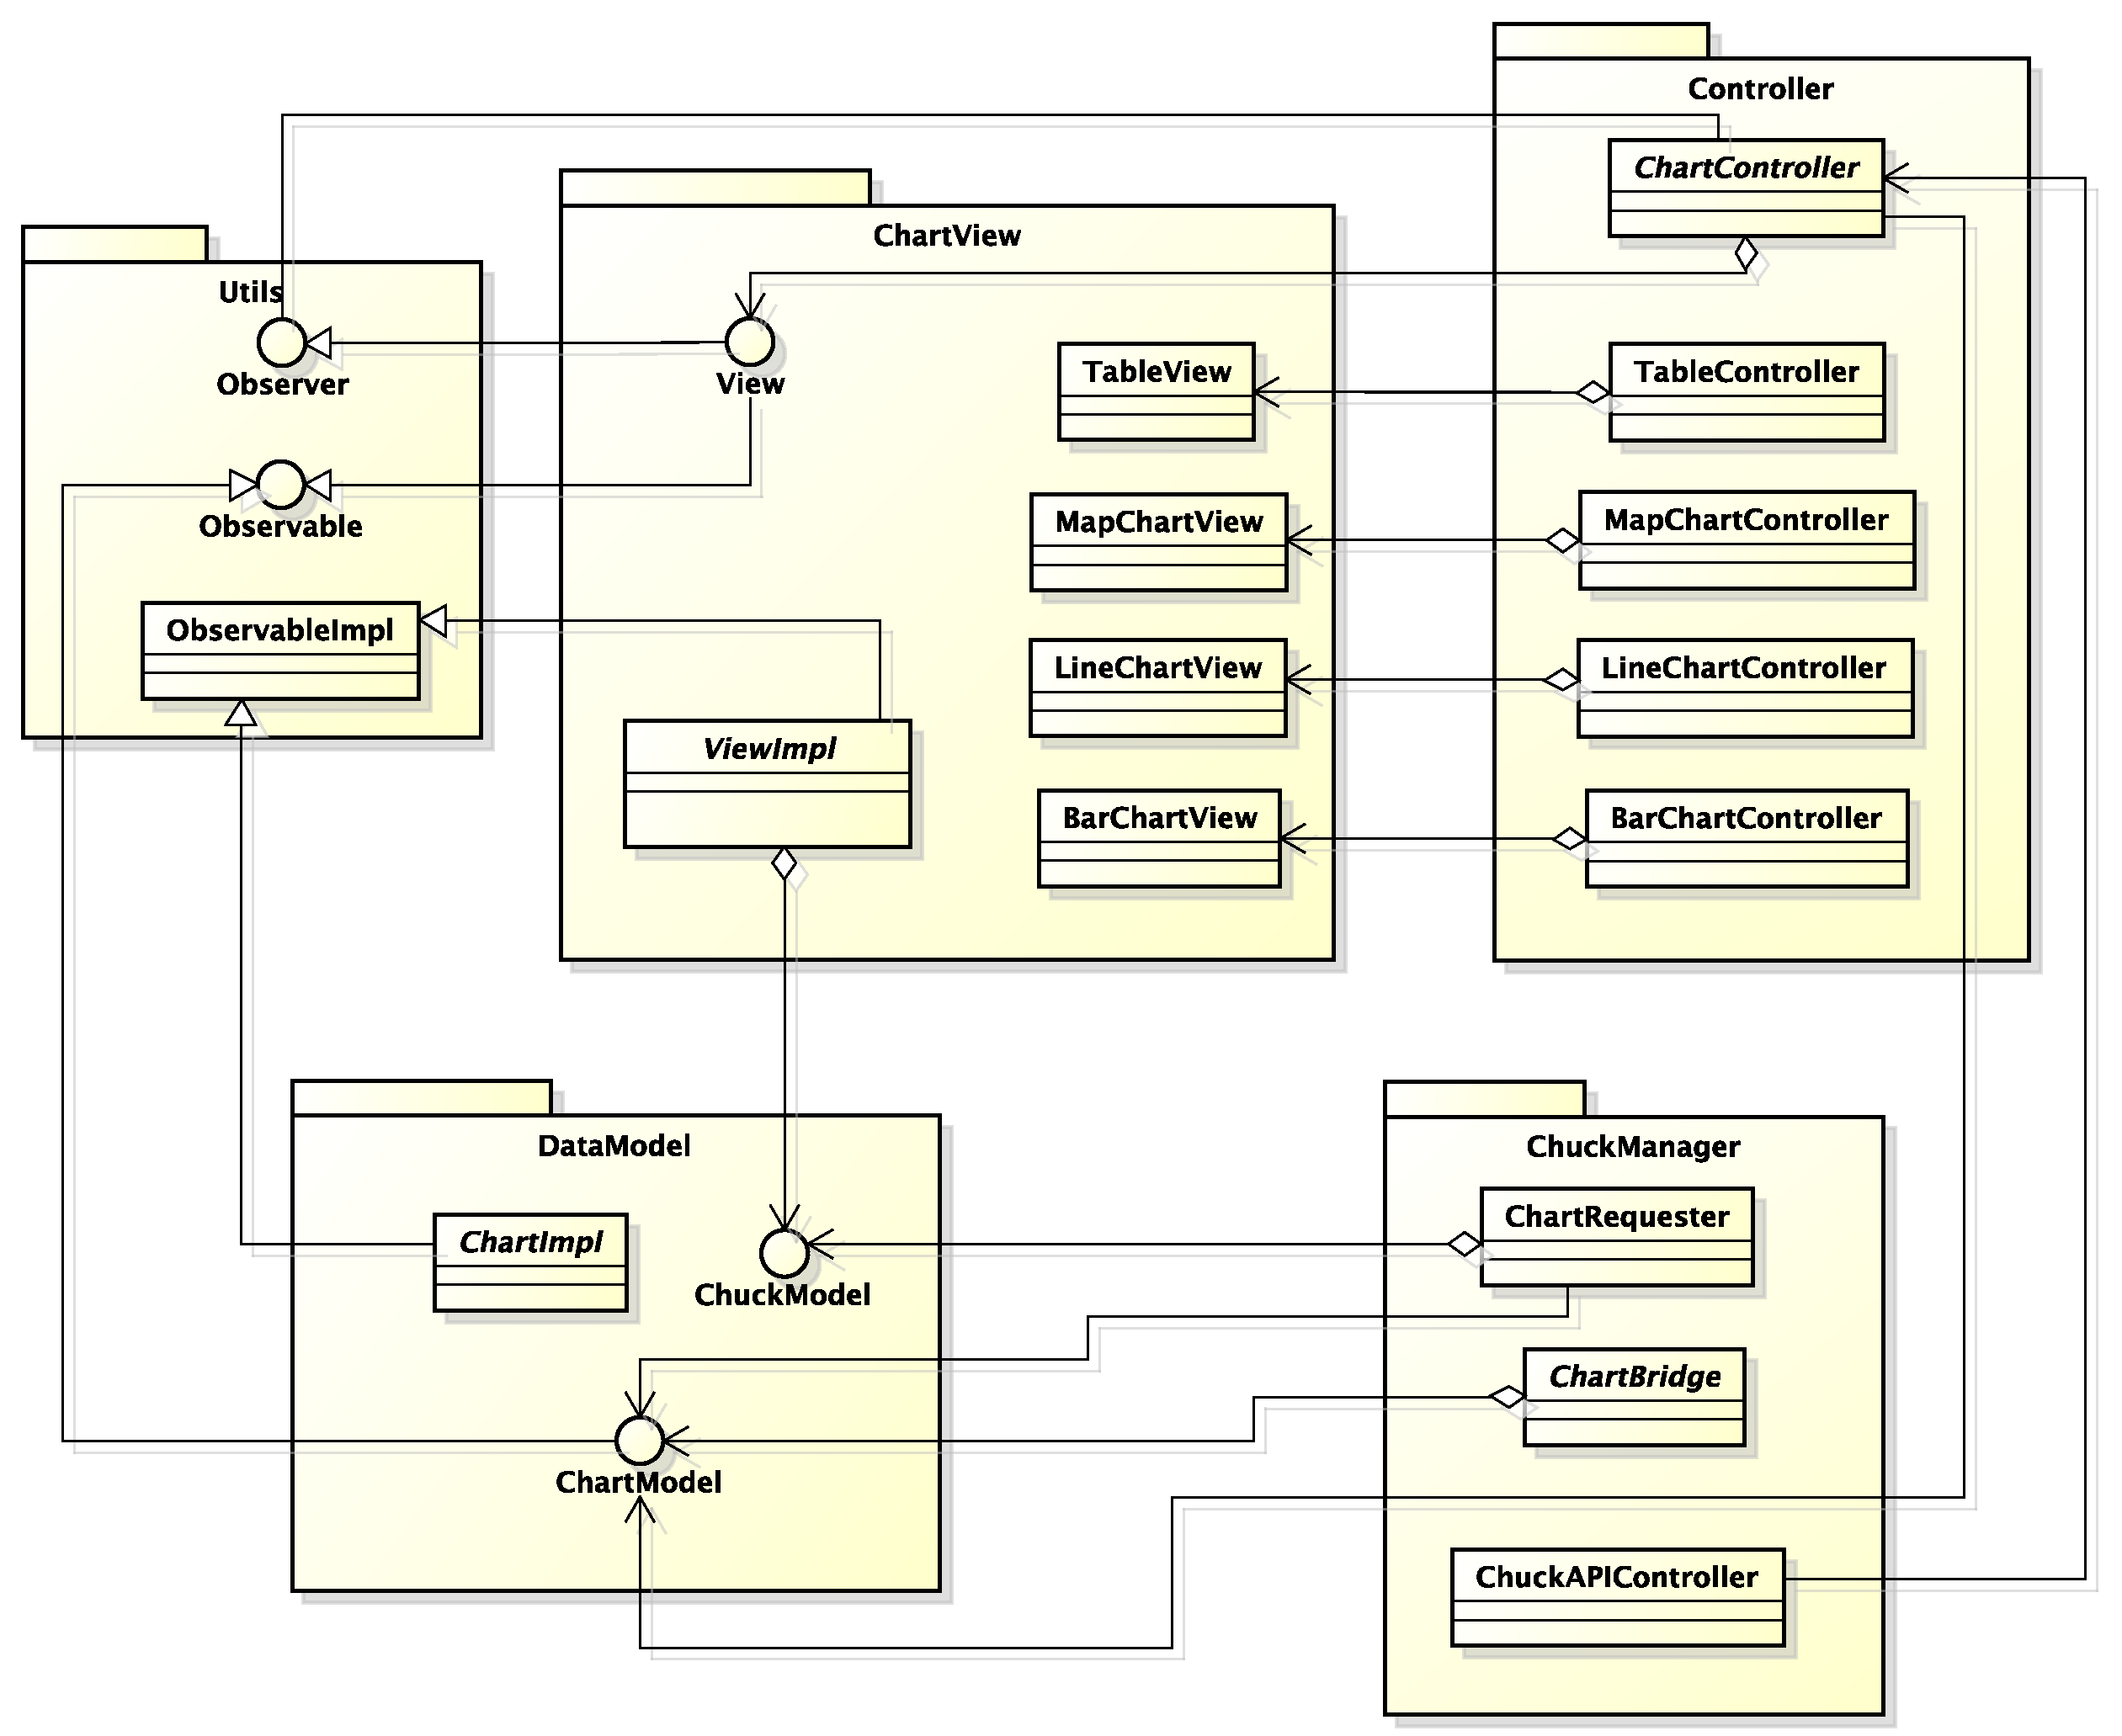
\includegraphics[width=\textwidth]{SpecificaTecnica/Pics/InterazioniComponentiChuck.pdf}
		\caption{Diagramma delle interazioni tra classi di componenti di Chuck}
	\end{figure}